\documentclass[12pt]{report}
\usepackage{polski}
\usepackage[utf8]{inputenc}
\usepackage{listings}
\usepackage{graphicx}

\linespread{1.3}
\usepackage[T1]{fontenc}
\usepackage{mathptmx}

\usepackage{geometry}

\graphicspath{ {./image/} }
\newgeometry{tmargin=2.5cm, bmargin=2.5cm, lmargin=3.5cm, rmargin=2.5cm}

\author{Tomasz Kowalczyk}
\title{Emulator procesora Zilog Z80}

\begin{document}
	\maketitle
	\tableofcontents
	
	\chapter{Wstęp}

	Celem pracy jest wykonanie emulatora procesora Zilog Z80. Aplikacja umożliwia wczytanie programu w postaci kodu maszynowego, deasemblację i wykonanie. Dostępne są dwa tryby wykonania: ciągły i krokowy. W obu przypadkach emulator obrazuje stan rejestrów, jak również umożliwia podgląd i zmianę zawartości pamięci programu. Aplikacja została zaimplementowana w języku Java.
	
	% to jest skopiowane prosto z książki
	Procesor Zilog z80 był szlagierem rynku mikroprocesorowego. \cite{karczmarczuk}
	Został wydany na rynek w roku 1976, i szybko zdominował rynek 8-bitowych procesorów.
	
	Jednym z jego powodów sukcesu na rynku, była prostota w sprzęganiu go z innymi urządzeniami, szczególnie pamięciami. Inną jego zaletą była lista rozkazów zgodna z popularnym w tamtym czasie procesorem, mianowicie Intelem 8086, co umożliwiało uruchamianie programów napisanych z pierwotnym przeznaczeniem dla Intela 8080 na Zilogu Z80. \cite{karczmarczuk}
	
	Urządzenie to mimo zalet, ma również jedną dużą wadę. Jego wewnętrzna budowa była złożona jak na tamte czasy, wyjścia nie były ułożone w logiczny sposób (widoczne na rysunku  \ref{img:z80wyprowadzenia}), a lista rozkazów składała się z 158 pozycji, w tym 78 z nich zgodnych z Intel 8080A \cite{manual}
	
	
	\begin{figure}[h]
		\centering
		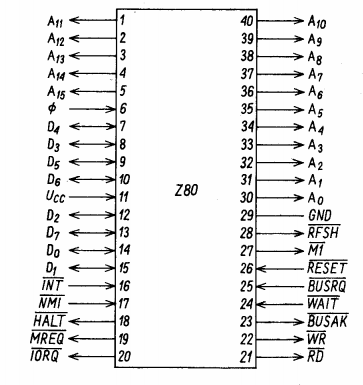
\includegraphics[width=1.0\textwidth]{z80wyprowadzenia}
		\caption{Wyprowadzenia mikroprocesora Z80}
		\label{img:z80wyprowadzenia}
	\end{figure}
			
	\begin{figure}[h]		
		\centering
		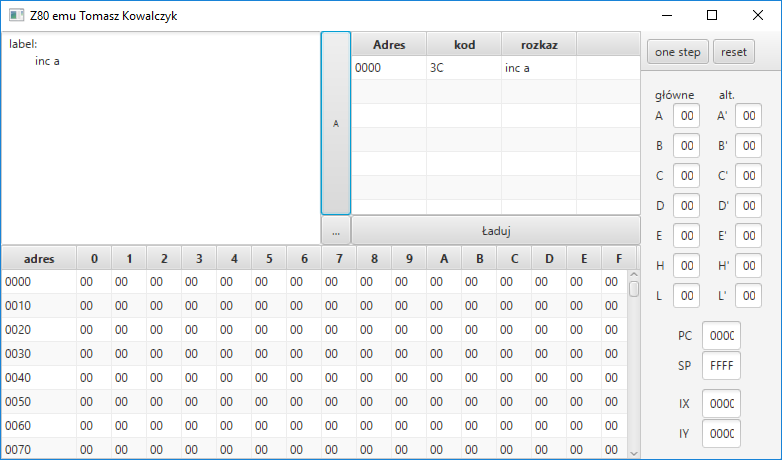
\includegraphics[width=1.0\textwidth]{app1}
		\caption{Widok główny emulatora}
	\end{figure}
	
	Samą aplikacje wykonano w języku Java 8 i biblioteki graficznej Java FX. 
	Interfejs użytkownika został podzielony na 3 części: 
	\begin{itemize}  
		\item widok kodu programu napisany w języku asembler, wraz z  wynikowym kodem maszynowym  
		\item widok pamięci w formie tabeli. Aby uzyskać adres odpowiadający danej komórce, należy dodać do siebie wartość \underline{?????}. Edycje wykonujemy przez dwukrotne kliknięcie w komórkę tabeli, wpisaniu nowej wartości i zatwierdzeniu klawiszem Enter.
		\item widok stanu wewnętrznych rejestrów procesora, wraz z przyciskami debugującymi.   
	\end{itemize}
	
	W aplikacji każda wyświetlona wartość podana jest w systemie heksadecymalnym, i także w takiej notacji wprowadzamy wartości (oprócz pola do edycji kodu asemblera, gdzie możemy używać innych notacji).
	
	\chapter{Zagadnienie emulacji}
	
	Emulator w kontekście informatyki, oznacza program który jest przystosowany do uruchomienia na specyficznym urządzeniu lub/i systemie, i pozwala na uruchomienie programów napisanych z przeznaczeniem dla innego urządzenia/systemu\cite{howDoIWriteAnEmulator}. 
	
	Inną ciekawą definicję emulatora podał Victor Moya del Barrio "Emulacja w informatyce oznacza emulowanie zachowania urządzenia lub oprogramowania za pomocą innego oprogramowania lub urządzenia"
	\cite{studyofthetechniquesforemulationprogramming}.
		
	Emulacje CPU można przeprowadzić na 3 sposoby:\cite{fms_komkon_org_howto}	
	\begin{itemize}  
		\item emulacja przez interpretowanie
		\item emulacja przez statyczną re-kompilacje
		\item emulacja przez dynamiczną re-kompilacje
	\end{itemize} 
	Każda z tych metod wymaga oddzielnego omówienia.
	
	\section{Emulacja przez interpretowanie}
	Interpreter to najprostszy rodzaj emulatora. Odczytuje w pętli kod programu z wirtualnej pamięci. Odczytany bajt (lub bajty, rozkaz procesora może być wielobajtowy) zawiera informacje o rodzaju operacji jaką CPU powinno wykonać. Interpreter ma za zadanie odkodować informacje o operacji, a następnie ją wykonać. Między kolejnymi rozkazami powinien on zmienić wirtualne parametry (np inkrementacja licznika rozkazów), sprawdzić czy nie zostało wywołane przerwanie, obsłużyć urządzenia wejścia/wyjścia, liczniki, kartę graficzną, lub wykonać inne operacje zależne od emulowanego urządzenia. Przykładowa struktura interpretera została przedstawiona w kodzie  \ref{listing:interpreter}
		
	\lstinputlisting[language=C, label={listing:interpreter}, caption={Przykładowa struktura interpretera procesora},captionpos=b]{listings/interpreter.c}
	
	Emulacja przez interpretowanie jest najwolniejszą formą emulacji, ale także najłatwiejszą w debugowaniu. Pozwala na prześledzenie wykonania operacji, i podgląd wewnętrznych stanów urządzenia. Z tego powodu jest najczęściej wybierana w debuggerach procesorów, mikro-kontrolerów dla programistów.
	
	\section{Statyczna re-kompilacja}
	Statyczna re-kompilacja (ang. "Static binary translation") to proces konwertowania kodu maszynowego na inny kod maszynowy przeznaczony dla docelowej architektury. Plik wykonywalny tłumaczony jest raz, za jednym podejściem przez cały plik. Problemem tego rozwiązania są instrukcje skoków pośrednich czyli takich gdzie adres skoku przechowywany jest w rejestrze lub pamięci, i może on być uzyskany tylko podczas wykonywania programu. W takim przypadku niemożliwym jest przetłumaczenie wszystkich instrukcji pliku wykonywalnego\cite{uqbt}. 
	
	
	\section{Dynamiczna re-kompilacja}
	Dynamiczna re-kompilacja (ang. "Dynamic binary translator"), w odróżnieniu od translacji dynamicznej, tłumaczy kod blokami, podczas jego wykonywania. Re-kompilacja występuje "na żądanie" co jest wolniejsze od statycznej re-kompilacji, ale rozwiązuje problem związany z statycznym tłumaczeniem kodu wykonywanego za instrukcjami skoków pośrednich.
	
	Raz przetłumaczony fragment kodu jest przechowywany w pamięci, na wypadek jego ponownego użycia, co pozwala zoptymalizować ten sposób emulacji\cite{uqbt}.
	
	
	Dynamicznej rekompilacji używa w dużym stopniu maszyna wirtualna javy. Wczesne wersje JVM (Java Virtual Machin) używały do swojego działania interpreterów, co okazało się mało wydajne. Dobrym sposobem na optymalizację maszyny wirtualnej okazało się dynamiczne tłumaczenie kodu maszynowego\cite{dynamicRecompilationInJava}. 
	
	
	
	\section{Różnica między symulacją a emulacją (i może virtualizacją???)} 
	coś o wirtualizacji http://jpc.sourceforge.net/oldsite/Emulation.html
	
	% Brakuje mi do tego bibliografii
	% linki z których czerpałem wiedze:
	% https://www.guru99.com/real-device-vs-emulator-testing-ultimate-showdown.html
	% http://fms.komkon.org/EMUL8/HOWTO.html
	% https://stackoverflow.com/questions/1584617/simulator-or-emulator-what-is-the-difference
	% https://www.quora.com/What-are-the-differences-between-simulation-and-emulation
	% TO NAJLEPSZE: https://softwareengineering.stackexchange.com/questions/134746/whats-the-difference-between-simulation-and-emulation
	Zagadnienie emulacji często mylone jest z symulacją. Nie są to jednak jednoznaczne pojęcia.
	
	W książe "Study of the techniques for emulation
	programming" Victor Moya del Barrio podaje taką to definicje emulatora "An emulator tries to duplicate the behaviour of a full computer using software programs in a different computer."\cite{studyofthetechniquesforemulationprogramming}. 
	\chapter{Przegląd istniejących rozwiązań}
	Zilog Z80 stał popularnym obiektem emulacji dzięki swojej popularności. Aplikacje te, pisano zarówno przez duże firmy, jak i hobbystów. Na jednej z usług hostingowych o nazwie ,,Github"  która jest przeznaczona dla projektów programistycznych, można znaleźć około 200 repozytoriów z projektami emulującymi Z80, lub emulującymi urządzenia używające tego procesora\cite{githubZ80Emulators}.   
	
	Poniżej zaprezentowane są najciekawsze pozycje tych programów, które posiadają graficzny interfejs użytkownika, i pozwalają na wgląd w  wewnętrzne stany procesora (czyli najbardziej przypominające zakresem swoich funkcji opisywany projekt). Przedstawiane są zarówno komercyjne rozwiązania, jak i te pisane przez amatorów.
	
	\section{Z80 SIMULATOR IDE}
	Dostępny pod adresem http://www.oshonsoft.com/z80.html płatny symulator posiadający najbardziej rozbudowany interfejs z wszystkich wymienionych pozycji. Pozwala on na prezentowanie wewnętrznych stanów procesora, manipulację przerwaniami, edytor pamięci umożliwiający działający również podczas symulacji, podgląd i manipulacja portami wejścia/wyjścia. Posiada również funkcje typowe dla debuggerów, możliwość wstrzymania działania programu w określonym miejscu, tryb pracy krokowej, interaktywny edytor i kompilator kodu asemblera\cite{oshonsoftEmulator}. Część funkcji została zaprezentowana na rysunku \ref{img:oshonsoftEmulator} 
	
	\begin{figure}[h]
		\centering
		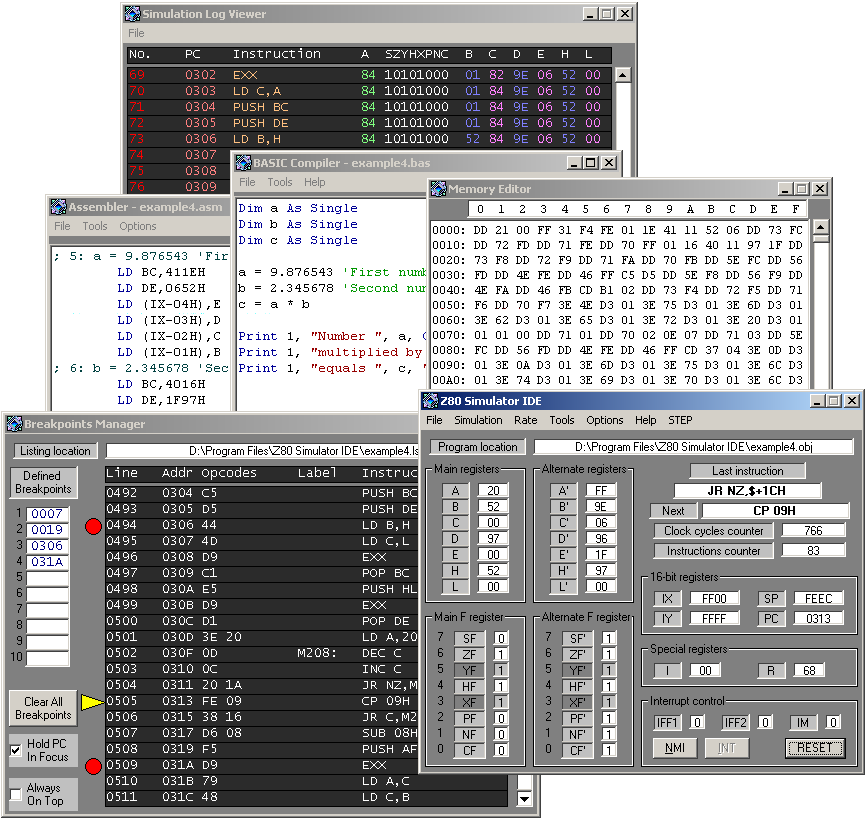
\includegraphics[width=0.7\textwidth]{oshonsoftEmulator}
		\caption{Z80 SIMULATOR IDE \cite{oshonsoftEmulator}}
		\label{img:oshonsoftEmulator}
	\end{figure}
	
	Jedną z wad emulatora jest interfejs, który nie jest intuicyjny. Dla przykładu, w żadnym miejscu nie znajdziemy informacji, o tym w jakim formacie powinny być wprowadzane wartości liczbowe. Brak w programie systemu pomocy i opisów, co może odstraszyć początkującego użytkownika. Dodatkowo jest to rozwiązanie płatne i przeznaczone tylko dla platformy MS Windows. Jest to narzędzie głównie dla specjalistów.
	
	
	\section{ZEMU - Z80 Emulator Joe Moore}
	ZEMU to emulator zaprojektowany głównie, do uruchamiania systemu CPM. Była to seria systemów operacyjnych oferowana przez firmę Digital Research Inc i latach 1970-1980\cite{cpm}.
	
	Program skierowany jest do hobbystów. Oprócz standardowych możliwości takich jak podgląd, edycja pamięci, rejestrów i flag, ma możliwość emulacji stacji dyskietek, portu COM, portu szeregowego, monitora CRT, drukarki.    
	
	Na rysunku \ref{img:zemu} przedstawiono interfejs aplikacji. Tak jak w przypadku Z80 SIMULATOR IDE nie jest intuicyjny, brak mu systemu pomocy, elementy interfejsu nie są opisane w wystarczającym stopniu. Osoby nie mające doświadczenia z urządzeniami wejścia/wyjścia w Zilogu Z80 będą miały problem z obsługą nawet podstawowych funkcji.
	
	Inną wadą aplikacji jest możliwość jej uruchomienia tylko w systemie Windows. 
	
	\begin{figure}[h]		
		\centering
		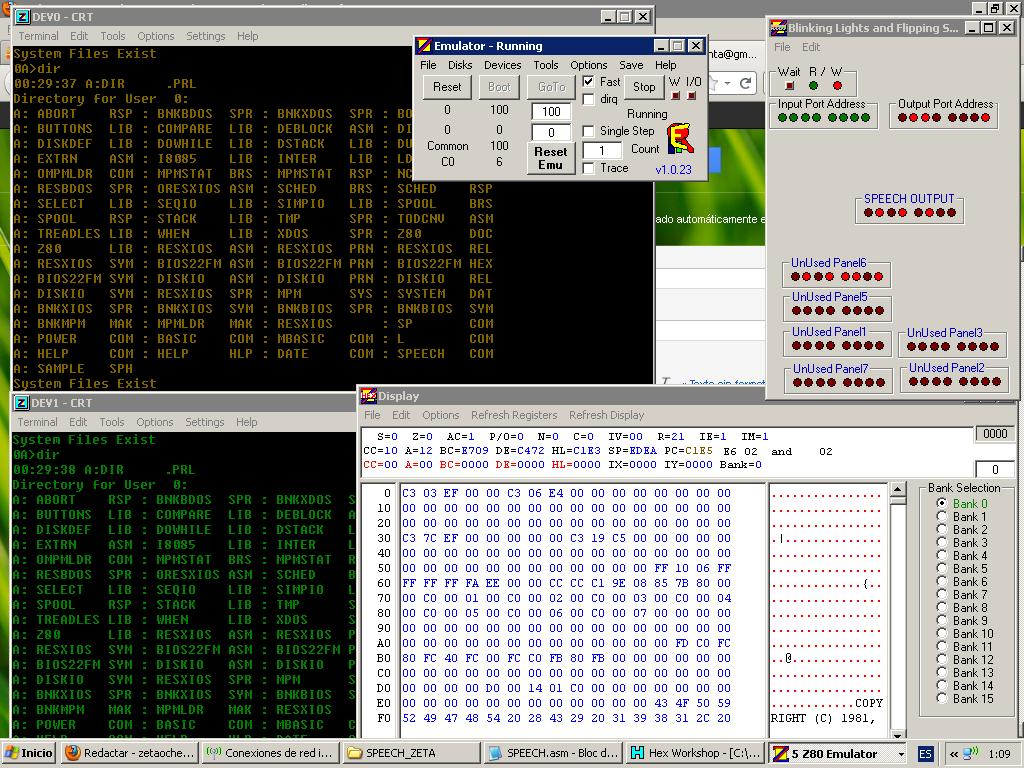
\includegraphics[width=0.8\textwidth]{zemu}
		\caption{ZEMU \cite{zemuImg}}
		\label{img:zemu}
	\end{figure}
	
	 \section{ZIM - The Z80 Machine Simulator}
	ZIM został napisany za pomocą technologi Java Web-Start. Pozwala to na uruchomienie aplikacji bezpośrednio na stronie internetowej, wraz z dostępem do lokalnych zasobów systemu, np plików\cite{zim}. 
	Aplikacja według autora przeznaczona jest głównie dla studentów uczących się języka asemblera dla procesora Z80\cite{zimPurpose}.
	
	Aplikacja pozwala na podgląd wszystkich wewnętrznych parametrów cpu, emuluje proste urządzenia wejścia/wyjścia, umożliwia edycję pamięci, debugowanie programu, symulację przerwań. Zaletą programu jest jego wieloplatformowość dzięki zastosowaniu języka Java.
	
	Brakuje w niej natomiast edytora asemblera, systemu pomocy, interfejs ma wiele błędów i nie jest intuicyjny. Na rysunku \ref{img:zim} przedstawiono zrzut ekranu działającej aplikacji.
	
	\begin{figure}[h]		
		\centering
		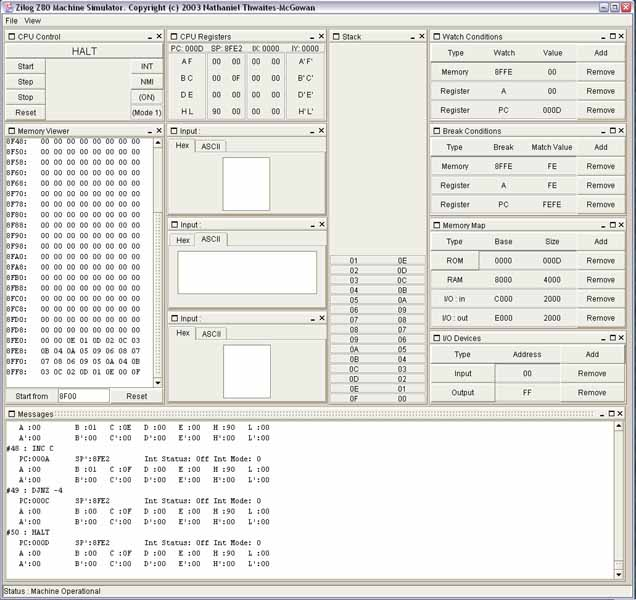
\includegraphics[width=0.8\textwidth]{zim}
		\caption{ZIM - The Z80 Machine Simulator \cite{zimImg}}
		\label{img:zim}
	\end{figure}
	
	%Żadne istniejące rozwiązanie nie pozwala na podejrzenie wewnętrznych magistrali procesora
	
	\section{Podsumowanie istniejących rozwiązań}
	Problemem prawie wszystkich emulatorów i symulatorów jest interfejs. Nie tyczy się to konkretnie omawianego procesora, ale ogółu tego typu aplikacji. Są one przeznaczone dla osób znających architekturę komputerową, oraz budowę i działanie konkretnego emulowanego urządzenia, z tego powodu programiści nie przywiązują do intuicyjności i systemów pomocy odpowiedniej wagi. Osoby nie posiadające wymaganej wiedzy, albo znające jedynie podstawy nie są w stanie sprawnie obsługiwać programu. 
	
	Emulatory rzadko są wielplatformowe. Dotyczy się to szczególnie aplikacji emulujących przez re-kompilacje. Aby ją wykonać wymagana jest znajomość architektur wyjściowej i docelowej. Rozwiązaniem tego problemu mogą być interpretery napisane w języku Java, tak jak "ZIM - The Z80 Machine Simulator". Rozwiązanie to wykorzystuje dużo zasobów procesora, kod emulowanej architektury jest najpierw interpretowany przez interpreter napisany w języku Java, a następnie ponownie emulowany już przez dynamiczną re-kompilacje w maszynie wirtualnej. Typowe rozwiązania napisane w języku kompilowanym pod konkretny procesor działają szybciej, kosztem wieloplatformowość. Optymalizacja w sprzęcie typu Zilog Z80 nie jest kluczową kwestią, współczesne komputery są na tyle szybkie, aby uruchomić emulator maszyny z lat 70 napisanej w Javie. 
	
	Kolejną kwestią o której warto wspomnieć jest czytelność kodu. Kod istniejących rozwiązań nie należy do przejrzystych, najczęściej cały kod emulatora zawiera się w jednym pliku z kilkuset liniami. Osoba pragnąca wgłębić się w sam proces emulacji w takim przypadku ma utrudnione zadanie.
	
	Podsumowując, aktualnie brakuje wieloplatformowego emulatora lub symulatora Ziloga Z80, z czytelnym, poprawnie działającym interfejsem, przejrzystym dobrze komentowanym kodem źródłowym, i system pomocy.
	
	
	\chapter{Projekt aplikacji}
	% uml-e, mvc. wzorce projektowe, może maven i javaDoc????????
	
	\section{Podział aplikacji}
	Aplikację podzielono na 3 mniejsze moduły, xbit, z80emu-core oraz z80emu-gui z czego każdy z nich jest osobnym mniejszym projektem, który używa narzędzia ,,Maven" do zautomatyzowania procesu budowy oprogramowania. Ich pliki jar są przetrzymywane w platformie mymavenrepo.com jako prywatne repozytorium, zabezpieczone hasłem przy pomocy funkcji protokołu http "basic auth". Każdy z projektów może zostać wysłany do zdalnego serwera za pomocą komendy ,,mvn deploy:deploy". Komenda ta przeprowadza testy jednostkowe, kompiluje kod javy do kodu bajtowego JVM, dodaje zewnętrzne bliblioteki jar i umieszcza plik wykonywalny na serwerze.
	
	Aby umożliwić integracje z serwisem mymavenrepo.com pliki pom.xml zawierają wpisy zaprezentowane w fragmencie kodu \ref{listing:myMavenRepoPom}. Ponieważ repozytoria maven są ustawione jako prywatne, należy odnaleźć w systemie plik ~/.m2/settings.xml podać w nim dane pozwalające na autoryzacje za pomocą "http basic auth". Przykład konfiguracji przedstawiono w kodzie \ref{listing:myMavenRepoSettings}
	
	\lstinputlisting[language=xml, label={listing:myMavenRepoPom}, caption={fragment pliku pom.xml umożliwający integracje z serwisem myMavenRepo},captionpos=b]{listings/myMavenRepoPom.xml}
	
	\lstinputlisting[language=xml, label={listing:myMavenRepoSettings}, caption={fragment pliku settings.xml przechowującego dane utoryzacyjne do serwera myMavenRepo},captionpos=b]{listings/myMavenRepoSettings.xml}
	
	Przetrzymywanie plików wykonywalnych w zewnętrznym serwisie ułatwia zarządzanie wszystkimi trzema projektami, pozwala na ich wersjonowanie, i łatwiejsze budowanie aplikacji. 

	\section{XBit}
	Java jest językiem programowania wysokiego poziomu, kompilowanym do kodu bajtowego. Z tego powodu nie jest on zazwyczaj stosowany w emulacji, gdyż kod emulatora musi być uruchamiany w maszynie wirtualnej, co nie należy do optymalnych rozwiązań.
	
	Innym poważnym problemem Javy jest brak typów danych przechowujących tylko wartości dodatnie. James Gosling, jeden z twórców Javy tak argumentuje ich brak: 
	,,Dla mnie jako projektant języków programowania, do których tak naprawdę ostatnimi czasy się nie zaliczam, coś prostego oznaczało skończenie na założeniu że losowy deweloper będzie w stanie zapamiętać specyfikacje. 
	Ta definicja mówi, że na przykład Java i wiele innych języków nie są proste, i w rzeczywistości wiele języków kończy z funkcjonalnościami których do końca nikt nie rozumie. Spytaj jakiegoś programistę języka C o dodatnie typy liczbowe, i odkryjesz że prawie żaden programista C faktycznie nie rozumie co dzieje się z typami bez znaku, czym jest arytmetyka liczb całkowitych. Takie rzeczy sprawiły że C jest językiem skomplikowanym. Myślę że w tej kwestii Java jest prosta"\cite{javaGoslingInterview}.
	
	Problem ten rozwiązano tworząc własną bibliotekę o roboczej nazwie XBit. Przechowuje ona liczby 8 i 16 bitowe, które mogą być interpretowane zarówno jako wartości całkowite jak i liczby w kodzie uzupełnień do dwóch. Biblioteka potrafi zwrócić konkretne bity, stworzyć reprezentacje liczby z pojedynczych bitów i typów prymitywnych, obudowuje operacje arytmetyczne z uwzględnieniem przepełnienia i przeniesienia. Kod projektu z jej użyciem staje się czytelniejszy i łatwiejszy do ewentualnej refaktoryzacji. 
	
	Bibliotekę zaprojektowano w taki sposób aby była możliwie jak najbardziej uniwersalna, i można ją było użyć nie tylko podczas emulacji Zilog-a Z80. ale także innych procesorów. 
	
	\subsection{Możliwości}
	Za cel obrano następujące funkcje:
	\begin{itemize}  
		\item odwzorowanie liczb 8 i 16 bitowych
		\item możliwość stworzenia reprezentacji liczb 8 i 16 bitowych z typów prymitywnych 
		\item interpretacja liczb w naturalnym kodzie binarnym lub dopełnień do dwóch
		\item operacje na pojedynczych bitach(możliwość zmiany, odczytu bitu o danym indeksie)
		\item opcja odczytania grupy bitów (odczytanie kilku bitów podając indeks pierwszego i ostatniego bitu)
		\item interpretacja liczb 16 bitowych w formacie big endian lub little endian
		\item operacje arytmetyczne (dodawanie, odejmowanie)
		\item operacje bitowe na liczbach (negacja, alternatywa, koniunkcja, przesunięcia bitowe)
		\item uwzględnienie przy operacjach arytmetycznych przepełnienia oraz przeniesienia
	\end{itemize} 
	
	\subsection{Założenia projektowe xBit}
	Przed przystąpieniem do implementacji rozwiązania, zaprojektowano publiczny interfejs biblioteki w języku uml, zaprezentowany na grafice \ref{img:xbitUml}. Ustalono także założenia projektowe które zaprezentowano poniżej. 
	
	\begin{figure}[h]
		\centering
		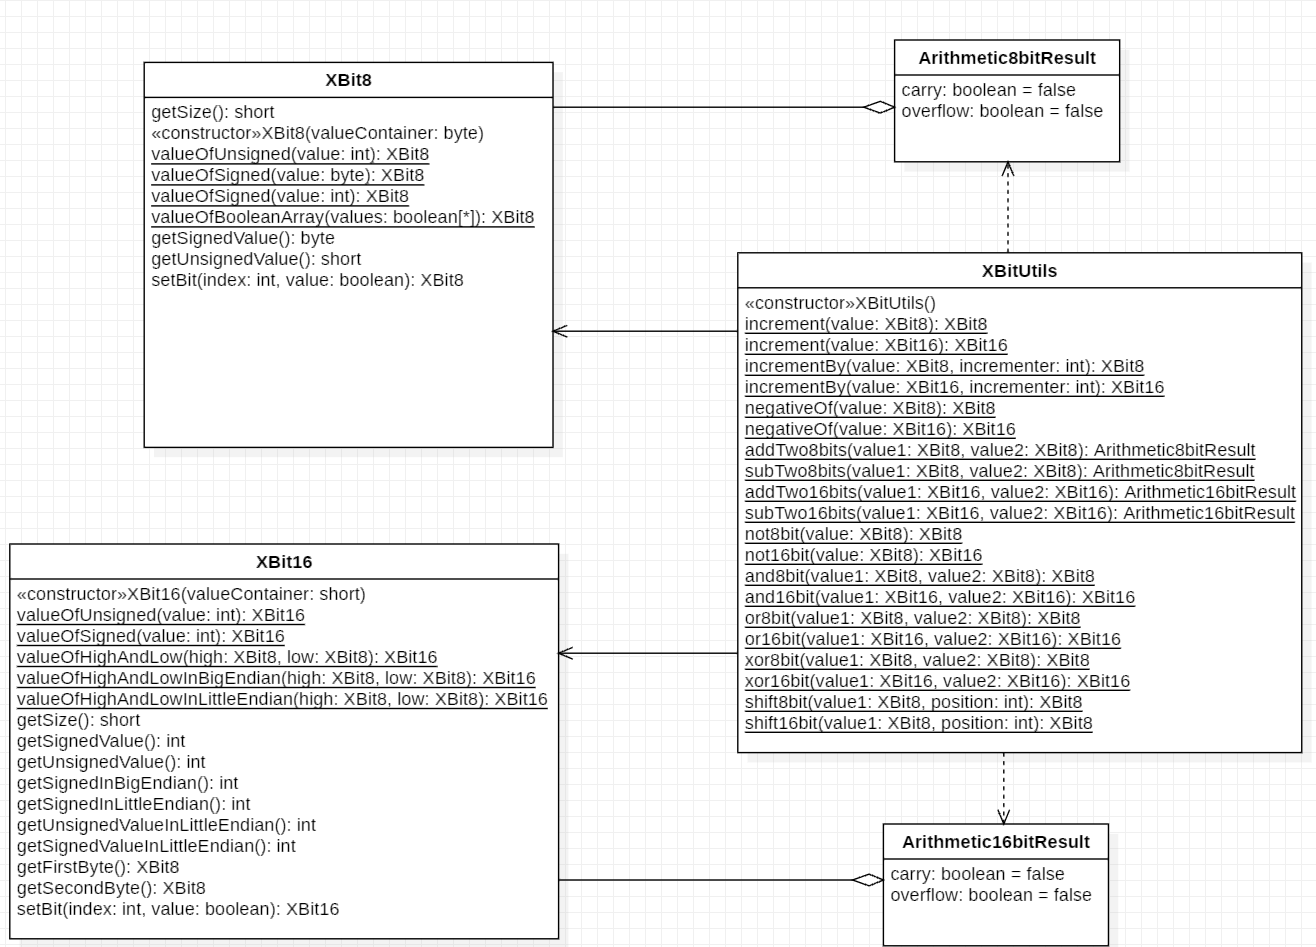
\includegraphics[width=1\textwidth]{xbitUml}
		\caption{projekt uml biblioteki xbit}
		\label{img:xbitUml}
	\end{figure}
	
	\subsubsection{Klasy XBit8 i XBit16}
	Klasy XBit8 oraz XBit16 to reprezentacje liczb 8 i 16 bitowych. Postanowiono, że nie będą one w stanie zmienić swojej wewnętrznej wartości, swego stanu (z angielskiego nazwano by je "immutable"), tak jak obiektowe reprezentacje typów prostych w javie (Short, Long, Integer itp).  Przez podjęcie tej decyzji projektowej, metody które powinny zmienić stan obiektu, klonują istniejący obiekt a następnie modyfikują odpowiednio jego stan. Przykładem takiej metody jest setBit(index: int, value: boolean) klasy Xbit8 oraz Xbit16. Funkcja ta nie zmienia bitu obiektu na rzecz którego została wykonana, a jedynie zwraca kopie obiektu, z zmodyfikowanym odpowiednim bitem. 
	
	Zalety zastosowania obiektów niezmiennych:
	\begin{itemize} 
		\item Prosta implementacja oraz łatwe debugowanie kodu.
		\item Garbage Collector jest zoptymalizowany pod względem pracy z tego typu obiektami.   
		\item Łatwość zapisywania obiektów do pliku lub pamięci podręcznej (z ang. cache).
		\item Bezpieczne używanie obiektów niezmiennych w programach wielowątkowych, co umożliwiałoby emulacje potokowości CPU. Jeden wątek w takim przypadku mógłby być odpowiedzialny za jeden stopień potoku, np osobny wątek pobierał by instrukcje z pamięci, inny dekodował instrukcję, kolejny wykonywał i tak dalej.
		\item Możliwość użycia obiektu jako klucz, np w HashMap. 
	\end{itemize}
	
	Wadą zastosowania obiektów niezmiennych jest optymalizacja, i zwiększone użycie pamięci, co mimo wszystko nie powinno być przeszkodą dla współczesnych komputerów. Ze względu na przewagę zalet w stosunku do jednej wady postanowiono użyć obiektów niezmiennych w bibliotece.
	
	\subsubsection{Klasa XBitUtils, Arithmetic8bitResult, Arithmetic16bitResult}
	Klasa XBitUtils jest odpowiedzialna za wszystkie operacje arytmetyczne oraz bitowe. Większość z jej metod zwraca obiekty klas XBit8 lub XBit16. Wyjątkami są metody wykonujące dodawanie lub odejmowanie, które oprócz zwrócenia wyniku operacji powinny informować o wystąpieniu przeniesienia lub przepełnienia. Z tego zaprojektowano  klasy Arithmetic8bitResult oraz Arithmetic16bitResult które zawierają następujące pola:
	\begin{itemize}
		\item obiekt klasy XBit8 lub XBit16 będący rezultatem operacji
		\item dwie zmienne typu boolean informujące o wystąpieniu przeniesienia i przepełnienia
	\end{itemize}
		
	
	
	\section{z80emu-core}
	Z80emu-core to moduł mający za zadanie wykonywać emulację oraz udostępniać zestaw metod umożliwiający  manipulacje tym procesem. Za cel obrano stworzenie takiego interfejsu, który pozwalał by na użycie Z80emu-core w innych projektach, które emulują urządzenia zbudowane między innymi z Ziloga Z80. Jako przykład można podać emulator przenośnej konsoli Game Boy firmy Nintendo z 1989 roku która jako główny procesor używała Ziloga Z80. 

	Za cel obrałem implementacje następujących funkcji:
	\begin{itemize}  
		\item możliwość wykonania wszystkich 158 instrukcji procesora
		\item zestaw metod umożliwiających zmianę stanów rejestrów
		\item emulacja zewnętrznej pamięci
		\item możliwość podłączenia urządzeń wejścia/wyjścia
		\item wywołanie przerwania maskowanego oraz niemaskowanego (Z80 posiada dwa rodzaje przerwań)
	\end{itemize}
	
	\subsection{Publiczny interfejs modułu z80emu-core}
	Publiczny zestaw metod służący manipulacją samym procesem emulacji jak i urządzeniem pokazano na grafice \ref{img:z80emuCoreUml}. Cała mechanika działania modułu została ukryta w trzech klasach: Z80, RegistersBank i DuplicableRegisterSet. 
	
	Klasa Z80 zawiera zestaw funkcji manipulującymi samą emulacją, oraz wartościami liczników i mniejszych rejestrów procesora. Niżej opisuje najważniejsze z nich:
	\begin{itemize}  
		\item Z80(memory: Memory, ioDevice: IoDevice) - konstruktor, przyjmujący dwa parametry wymagane do poprawnego działania. Parametr ,,memory" oraz "ioDevice to obiekty implementujące interfejsy o tych samych nazwach. Reprezentują one kolejno moduł pamięci oraz urządzenia wejścia wyjścia podłączone do procesora. Użytkownik używający modułu Z80emu-core ma powinien samemu zaimplementować ich działanie, z zależności od otoczenia w jakim chce emulować urządzenie. 
		
		\item runOneInstruction() - metoda wykonująca jedną instrukcję procesora, za jej pomocą wykonane zostanie pobieranie, dekodowanie, wykonywanie rozkazu, ale również obsługa przerwań, inkrementacja liczników.
		
		\item makeInterupt(addressBus: XBit8), makeNonMaskableInterupt(addressBus: XBit8) - metody powinny zostać wywołane między kolejnymi wywołaniami runOneInstruction(). Ich zadaniem jest zgłaszanie przerwań. Parametr addressBus to wartość jaka została by ustalona na magistrali danych podczas przerwania, gdyby zostało ono wykonane w prawdziwym urządzeniu.
	\end{itemize}
	
	Wartym przypomnienia jest, że Zilog Z80 jest procesorem posiadającym dwa zestawy rejestrów ogólnego przeznaczenia (do nich należąc rejestry A,B,C,D,E,H,L,F oraz ich 16bitowe odpowiedniki). Takie rozwiązanie jest optymalne, w przypadku gdy procesor często wykonuje obsługę przerwań. W klasycznym podejściu, podczas przerwania zestawi rejestrów ogólnego przeznaczenia zapisany zostałby na stosie, co jest czasochłonną operacją. Projektanci Ziloga Z80 postanowili stworzyć drugi alternatywny zestaw rejestrów ogólnego przeznaczenia, który zostaje przełączony jako główny podczas przerwania. W takim przypadku nie jest wymagane odłożenie wartości na stos.
	
	W projekcie reprezentacją zestawu rejestrów ogólnego przeznaczenia jest klasa DuplicableRegisterSet. Jej dwie instancje (jedna jako główny zestaw rejestrów, druga alternatywny) przechowuje klasa RegisterBank, która posiada metody switchRegisterSet(), switchRegisterSetToA() i switchRegisterSetToB() pozwalające na przełączanie głównego zestawu rejestrów. Metody typu getA(), setA(value: XBit8) to aliasy wykonujące te operacje na aktualnie aktywnym zestawie. 
	
		
	
	\begin{figure}[h]
		\centering
		\includegraphics[width=1\textwidth]{z80EmuCoreUml}
		\caption{publiczny interfejs projektu z80emu-core zaprezentowany za pomocą diagramu klas uml}
		\label{img:z80emuCoreUml}
	\end{figure}
	
	\subsection{przerwania}
	
	Postanowiono nie tworzyć samej emulacji w nowym wątku, oraz nie uruchamiać jej w pętli głównej tak jak w klasycznym podejściu pokazanym w kodzie \ref{listing:interpreter}. Zamiast tego udostępniono jedną metodę runOneInstruction() : void która uruchamia jeden rozkaz procesora, uwzględniając czy wcześniej nie zostały wywołane metody makeInterrupt(addressBus : XBit8), makeNonMaskableInterrupt(addressBus : XBit8), resett(addressBus : XBit8)
	
	%Pamięć fizycznie jest zewnętrznym modułem, mimo to uwzględniono jego implementację w projekcie aplikacji. 
	
	\section{z80emu-gui}
	%tutaj o mvc
	
	
	\chapter{Implementacja}
	fragmenty kodu, podział na pakiety	
	\chapter{Testy}
		
	\section{????}
	Bardzo ważną kwestią w projekcie było dokładne pokrycie kodu aplikacji w testach jednostkowych. Emulator mikro-kontrolera to specyficzna aplikacja. Z pozoru mało znaczący błąd może sprawić że emulator stanie się bezużyteczny. 
	
	Dla przykładu, jeśli dla 3 bajtowego rozkazu procesora zwiększymy rejestr PC o 2 zamiast o 3, to nie wykona się następna instrukcja przewidziana przez programistę. Dalsza praca emulatora stanie się nieprzewidywalna, a następna instrukcja całkowicie “wykolei” nasz program który zacznie wykonywać losowe instrukcje. 
	
	Dlatego poprawne wykonanie każdego rozkazu jest tak ważne dla mojego projektu. Aby uchronić się przed tego typu prostymi błędami każdy emulowany rozkaz posiada swój test/testy jednostkowe napisane przy pomocy biblioteki Junit. 
	
	Przykładowy test dla rozkazu LD A, I. Rozkaz ten ładuje zawartość rejestru A z I:
	\lstinputlisting[language=Java]{listings/exampleTest.java}
	
	Opisany przykład ukazuje że prosta z pozoru operacja jak pobranie wartości jednego rejestru i przeniesienie go do innego, wymaga objętościowych testów. Oprócz testowania czy poprawna wartość znajduje się w rejestrze docelowym, musimy sprawdzić także czy flagi CPU zostały ustawione na poprawnych wartościach, czy ilość przewidywanych cykli zegara została poprawnie zwiększona, czy rejestr PC został zainkrementowany. 
	
	\section{Test-driven development}
	TDD to metoda pisania oprogramowania. Zakłada ona że test jednostkowy dla danej funkcjonalności powstaje jako pierwszy. Dopiero po napisaniu testu implementujemy kod programu, a następnie testujemy za pomocą już napisanych testów. Za pomocą TDD była pisana cała aplikacja	
	\chapter{Uwagi i wnioski}
	
	Z  wymienionych celów, nie zrealizowałem jedynie emulacji wewnętrznych magistrali procesora. Nie posiadając dokumentacji technicznych opisujących wewnętrzną budowę mikroprocesora, jedyną opcją było by poddanie urządzenia inżynierii wstecznej, \underline{co już nie jest tematem tej pracy.}
	
	% zmiana implementacji z valueContainer na ByteBuffer dla XBit
	
	
	
	
	
	
	\begin{thebibliography}{9}
		\bibitem{studyofthetechniquesforemulationprogramming}
		Victor Moya del Barrio
		\emph{Study of the techniques for emulation programming}.
		2001
		
		\bibitem{fms_komkon_org_howto}
		http://fms.komkon.org/EMUL8/HOWTO.html
		
		\bibitem{karczmarczuk}
		Mikroprocesor Z80 Jerzy Karczmarczuk
		
		\bibitem{manual} 
		Oficjalny manual
		
		\bibitem{howDoIWriteAnEmulator} https://www.atarihq.com/danb/files/emu\_vol1.txt
		How do I write an emulator? Daniel Boris, 1999
	\end{thebibliography}
	
\end{document}